% COMS 6998, Fall 2026 -- P1: Exploration & Progress
% Build: latexmk -pdf neural-symbolic-p1.tex
% Evidence: PROGRESS.md, results/p1/ and results/p2/ in the ReasonLink repository.
% Two pages of main content; references follow directly after the body.
\documentclass[conference,10pt,letterpaper]{IEEEtran}
\usepackage[T1]{fontenc}
\usepackage{cite}
\usepackage{amsmath,amssymb}
\usepackage{booktabs}
\usepackage{tabularx}
\usepackage{balance}
\usepackage{graphicx}
\usepackage{tikz}
\usetikzlibrary{arrows.meta}
\usepackage{pgfplots}
\pgfplotsset{compat=1.18}
\newcommand{\baselineDataFile}{figures/baseline-walltime.tsv}
\usepackage[hyphens]{url}
\usepackage[hidelinks]{hyperref}
\newcolumntype{Y}{>{\raggedright\arraybackslash}X}

\title{ReasonLink: Characterizing and Optimizing the\\Handoff Between Neural and Symbolic Accelerators}
\author{\IEEEauthorblockN{Vayun Gupta (vg2684), Aaron Mano Cherian (amc2535)}
\IEEEauthorblockA{COMS 6998: AI-Native Computing $\mid$ Fall 2026\\
P1: Exploration \& Progress $\mid$ Due October 26, 2026, 11:59 PM ET}}

\begin{document}
\maketitle
\thispagestyle{plain}
\pagestyle{plain}

\section{Project Direction and Updates}
Neurosymbolic AI is an emerging compositional paradigm that fuses neural learning with symbolic reasoning to enhance the transparency, interpretability, and trustworthiness of
AI. It also exhibits higher data efficiency making it promising for edge deployments \cite{cogsys}. Because the neural stage is compute bound, and the symbolic stage is memory bound, heteregenous hardware deployment, such as a specialized accelerator for each stage, is a natural fit. 
However, the interface between the two accelerators can become a bottleneck, limiting end-to-end performance. 

We therefore ask: \emph{after both ends of a neuro-symbolic pipeline are accelerated, does the interface between them become the bottleneck, and if so, which interface mechanisms remove it?} 

In visual Sudoku, a neural network reads the given digits and a SAT solver completes the grid~\cite{satnet}. SAT-Accel's host interface~\cite{sataccel} requires the CPU to rebuild and transfer roughly 632\,KB of solver data per puzzle, including the unchanged Sudoku rules and their metadata. In our lean serial software baseline, the solver waits about 0.71\,ms for this preparation before the MiniSat backend runs for another 0.73\,ms.

ReasonLink aims to replace this repeated image construction with compact solver-native literals and reusable base constraints, so inference and solver-input preparation can overlap. Predictions should enter the solver's input path as they are produced. The challenge is to manage buffer ownership and reset assignments and learned clauses between puzzles without corrupting the shared rules. Figure~\ref{fig:handoff-paths} shows the baseline and current design.

Since the proposal, we replaced Chipyard/Rocket/Gemmini with ESP~\cite{esp}/Ariane/NVDLA \emph{nv\_small} (int8) to use the available server toolchain and existing NVDLA integration. The server lacks \texttt{v++}/XRT, so we built a custom SAT-Accel integration and driver flow using Vitis HLS. To avoid building a combined tile, NVDLA and SAT-Accel remain separate and exchange data through DRAM. \emph{ReasonLink Milestone 1} reuses the base image in DRAM; \emph{Milestone 2} will keep the base on chip.

\section{Exploration and Findings}
\begin{figure*}[t]
\centering
\resizebox{\textwidth}{!}{% Compact report layout; detailed standalone layout is in
% reasonlink-baseline-comparison.tex. Both describe ReasonLink Milestone 1.
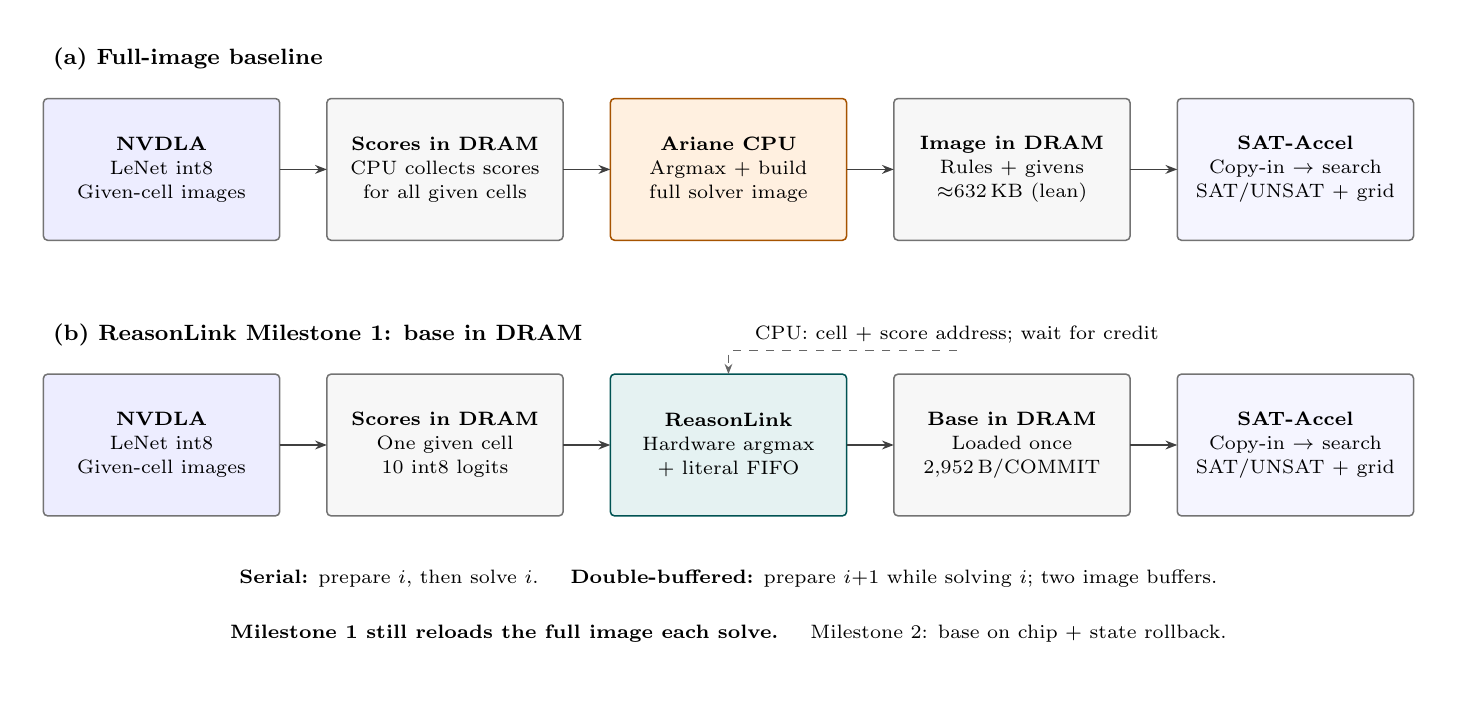
\begin{tikzpicture}[x=1mm,y=1mm,
  font=\fontsize{7.5}{8.7}\selectfont,
  block/.style={draw=black!55, rounded corners=1.5pt, line width=.55pt,
    align=center, minimum width=30mm, minimum height=18mm,
    inner sep=2pt, outer sep=0pt},
  neural/.style={block, fill=blue!7},
  memory/.style={block, fill=black!3},
  host/.style={block, fill=orange!12, draw=orange!65!black},
  rl/.style={block, fill=teal!10, draw=teal!65!black},
  solver/.style={block, fill=blue!4},
  data/.style={-{Stealth[length=1.5mm]}, line width=.65pt, draw=black!75},
  control/.style={-{Stealth[length=1.3mm]}, dashed, line width=.6pt,
    draw=black!60}
]
\path[use as bounding box] (0,-34) rectangle (179,49);
\node[anchor=west, font=\bfseries\fontsize{8.5}{10}\selectfont] at (2,45)
  {(a) Full-image baseline};
\node[neural] (bn) at (17,31)
  {\textbf{NVDLA}\\LeNet int8\\Given-cell images};
\node[memory] (bl) at (53,31)
  {\textbf{Scores in DRAM}\\CPU collects scores\\for all given cells};
\node[host] (bc) at (89,31)
  {\textbf{Ariane CPU}\\Argmax + build\\full solver image};
\node[memory] (bi) at (125,31)
  {\textbf{Image in DRAM}\\Rules + givens\\$\approx$632\,KB (lean)};
\node[solver] (bs) at (161,31)
  {\textbf{SAT-Accel}\\Copy-in $\rightarrow$ search\\SAT/UNSAT + grid};
\draw[data] (bn) -- (bl);
\draw[data] (bl) -- (bc);
\draw[data] (bc) -- (bi);
\draw[data] (bi) -- (bs);

\node[anchor=west, font=\bfseries\fontsize{8.5}{10}\selectfont] at (2,10)
  {(b) ReasonLink Milestone 1: base in DRAM};
\node[font=\fontsize{7}{8}\selectfont] at (118,10)
  {CPU: cell + score address; wait for credit};
\node[neural] (rn) at (17,-4)
  {\textbf{NVDLA}\\LeNet int8\\Given-cell images};
\node[memory] (rl) at (53,-4)
  {\textbf{Scores in DRAM}\\One given cell\\10 int8 logits};
\node[rl] (rc) at (89,-4)
  {\textbf{ReasonLink}\\Hardware argmax\\+ literal FIFO};
\node[memory] (ri) at (125,-4)
  {\textbf{Base in DRAM}\\Loaded once\\2,952\,B/COMMIT};
\node[solver] (rs) at (161,-4)
  {\textbf{SAT-Accel}\\Copy-in $\rightarrow$ search\\SAT/UNSAT + grid};
\draw[data] (rn) -- (rl);
\draw[data] (rl) -- (rc);
\draw[data] (rc) -- (ri);
\draw[data] (ri) -- (rs);
\draw[control] (118,8) -| (rc.north);

\node[font=\fontsize{7.2}{8.5}\selectfont] at (89,-21)
  {\textbf{Serial:} prepare $i$, then solve $i$. \quad
   \textbf{Double-buffered:} prepare $i{+}1$ while solving $i$; two image buffers.};
\node[font=\fontsize{7.2}{8.5}\selectfont] at (89,-28)
  {\textbf{Milestone 1 still reloads the full image each solve.} \quad
   Milestone 2: base on chip + state rollback.};
\end{tikzpicture}
}
\caption{ESP data paths. The baseline rebuilds the image every puzzle; ReasonLink Milestone 1 updates the fixed-decision array and counters (2,952\,B including padding). Solid arrows carry data; dashed arrows indicate CPU control. The software pilot replays scores with MiniSat; RTL tests replay scores with SAT-Accel.}
\label{fig:handoff-paths}
\end{figure*}

\textbf{Software optimization and overlap.} We compared serial and double-buffered paths using \emph{faithful} handling (clear and copy all 10.5\,MB of allocated buffers) and \emph{lean} handling (only the used regions, about 632\,KB). Double buffering prepares puzzle $i{+}1$ while solving puzzle $i$. The pilot uses replayed classifier scores and MiniSat~\cite{minisat} on x86 under WSL2.

\begin{figure}[t]
\centering
% Vector chart. Data: python3 generate-baseline-walltime.py
% Times are mean wall time per puzzle, not sums of phase medians.
\providecommand{\baselineDataFile}{baseline-walltime.tsv}
\begin{tikzpicture}
\begin{axis}[
  width=\linewidth,
  height=38mm,
  ybar=7pt,
  bar width=14pt,
  xmin=0.55, xmax=2.45,
  ymin=0, ymax=3.45,
  xtick={1,2},
  xticklabels={Faithful,Lean},
  ytick={0,1,2,3},
  ylabel={Wall time (ms/puzzle)},
  tick label style={font=\fontsize{8}{9}\selectfont},
  label style={font=\fontsize{8}{9}\selectfont},
  axis line style={black!55},
  axis x line*=bottom,
  axis y line*=left,
  ymajorgrids=true,
  grid style={black!12},
  tick align=outside,
  major tick length=2pt,
  legend style={at={(0.5,1.04)}, anchor=south,
    legend columns=2, draw=none, fill=none,
    font=\fontsize{8}{9}\selectfont,
    /tikz/every even column/.append style={column sep=5pt}},
  nodes near coords,
  every node near coord/.append style={
    font=\fontsize{7.5}{8.5}\selectfont,
    /pgf/number format/fixed,
    /pgf/number format/precision=3,
    /pgf/number format/fixed zerofill},
  clip=false,
]
\addplot[fill=blue!55!black,draw=blue!70!black]
  table[x=group,y=serial] {\baselineDataFile};
\addplot[fill=orange!70,draw=orange!80!black]
  table[x=group,y=double] {\baselineDataFile};
\legend{Serial,Double-buffered}
\end{axis}
\end{tikzpicture}

\caption{Average wall time over 1,000 puzzles after 20 warm-ups; one run per configuration. Replayed scores and MiniSat on x86. Lean double buffering provides $1.81\times$ throughput over lean serial execution.}
\label{fig:pilot}
\end{figure}

Lean handling reduces serial wall time from 2.81 to 1.45\,ms (Fig.~\ref{fig:pilot}). Argmax takes less than 1\,$\mu$s; image construction dominates conversion. Double buffering reduces lean wall time to 0.80\,ms, leaving only 5.1\% outside backend execution, but barely helps faithful mode. These results make lean double buffering a necessary comparison: overlap already hides most preparation in this pilot, while still rebuilding and copying the image.

\textbf{Base reuse.} The base formula has 729 variables and 11,988 clauses. Across 1,000 puzzles, only 1,212 image bytes (0.19\%) differ from the base on average. SAT-Accel already applies unit clauses as level-0 fixed decisions. Supplying givens this way on a reusable DRAM image preserves SAT/UNSAT results on 1000/1000 puzzles. We therefore include CPU-only delta updates to separate the benefit of base reuse from hardware literal generation.

\textbf{RTL loading cost.} ReasonLink Milestone 1 passes three RTL puzzles with reference results and unchanged search counts. Conversion takes 67 cycles per given and commit takes 1,181 cycles (Table~\ref{tab:rtl}). Across these cases, SAT-Accel busy cycles change by less than 0.2\%: it still reads about 650\,KB each solve. Milestone 1 removes CPU image construction but retains this loading cost. That motivates Milestone 2: keep the base on chip and roll back per-puzzle state.

\begin{table}[t]
\centering
\caption{RTL cycles at 100\,MHz; testbench memory has 30-cycle read latency and one burst at a time. Busy includes loading and search.}
\label{tab:rtl}
\footnotesize
\setlength{\tabcolsep}{3pt}
\begin{tabularx}{\columnwidth}{@{}Yrrrrr@{}}
\toprule
& & \multicolumn{2}{c}{\textbf{ReasonLink}} & \multicolumn{2}{c}{\textbf{SAT-Accel busy}} \\
\cmidrule(lr){3-4}\cmidrule(l){5-6}
\textbf{Puzzle} & Givens & Conv. & Commit & Baseline & RL \\
\midrule
0 (SAT) & 36 & 2,412 & 1,181 & 202,894 & 202,558 \\
3 (SAT) & 27 & 1,809 & 1,181 & 207,411 & 207,176 \\
5 (UNSAT) & 29 & 1,943 & 1,181 & 188,484 & 188,177 \\
\bottomrule
\end{tabularx}
\end{table}

\textbf{Workload limits.} Given-cell accuracy is 99.26\%, but only 79.0\% of puzzles recover the ground-truth grid; comparisons must hold predictions fixed. The current puzzles need only 1.17 mean MiniSat decisions, so harder instances are needed to test whether gains persist when search takes longer.

\newpage
\section{Implementation and Infrastructure Progress}
\textbf{Software.} We built 1,000 MNIST-based Sudoku puzzles, an int8 classifier emulator, a PySAT~\cite{pysat} reference, and the baseline harness. Retraining raised emulated MNIST accuracy from 74.5\% to 99.20\%; the NVDLA model compiles but awaits hardware validation. The C image builder matches SAT-Accel's host code byte for byte on 13 cases. All four pilot configurations agree on all 1,000 puzzles; eight solutions differ from the reference but satisfy their instances.

\textbf{Hardware.} Seven HLS kernels, a Vivado block design, APB/AXI shell, and C driver replace \texttt{v++}/XRT. We halved clause capacity to fit the VCU118. SAT-Accel passes 11 Sudoku and six other RTL cases. Its out-of-context netlist uses 112k LUTs and 434 URAMs (45\%), with $+$2.0\,ns post-synthesis slack at 10\,ns. ReasonLink Milestone 1 passes RTL tests but has no synthesized netlist yet.

\textbf{Integration and blockers.} The 2$\times$3 ESP SoC, Linux image, drivers, and board harness build. The harness passes host tests with a simulated device. Full-SoC simulation boots Ariane, discovers SAT-Accel, and loads an image; solve completion is pending. SoC synthesis passes, but an unlinked SAT-Accel checkpoint blocks bitstream implementation. No board timing or classifier-output validation is available. Code, results, and reproduction scripts are maintained in \href{https://github.com/AaronCherian404/ReasonLink}{the ReasonLink repository}.

\section{Next Steps}
\textbf{November 6 midterm.} Present the pipeline, software comparisons, and Milestone 1 RTL results. Fix checkpoint linking, build the baseline bitstream, then synthesize ReasonLink and build its bitstream. Repeat pilot measurements to assess variability.

\textbf{November 9 course P2.} Run full-image, CPU-delta, and ReasonLink handoffs, each serial and double-buffered, with NVDLA and SAT-Accel on the VCU118. Check logits against the emulator and report inference, conversion, transfer, synchronization, solver busy cycles, and puzzles/s. This will measure whether hardware improves on optimized software.

Then implement ReasonLink Milestone 2, validate state rollback across puzzles, and test harder instances. The December 18 final submission will include code, pinned environments, raw results, and reproduction scripts.

\clearpage
\bibliographystyle{IEEEtran}
\bibliography{neural-symbolic-references,p1-additional-references}
\end{document}
